\section{Diskussion der Ergebnisse}
\label{sec:diskussion}

\subsection{Fragen der Praktikumsanleitung}
\begin{enumerate}
	\item \textit{Welche Kerne sind mit der NMR-Spektroskopie detektierbar?}\vspace*{1mm}\\
	Mit der NMR-Spektroskopie sind g/u-Kerne, u/g-Kerne und u/u-Kerne detektierbar. Der erste Buchstabe steht in dieser Angabe für die Anzahl der Protonen im Kern, der zweite Buchstabe für die Anzahl an Neutronen. Charakterisiert werden beide Zahlen mit \textit{u} und \textit{g}, was für eine gerade oder ungerade Anzahl des jeweiligen Kernbausteins steht. 
	\item \textit{Welche Größen spielen für die Empfindlichkeit der NMR-Spektroskopie eine Rolle?}\vspace*{1mm}\\
	Die Empfindlichkeit der NMR-Spektroskopie hängt von den folgenden Größen ab:
	\begin{itemize}
		\item Häufigkeit des Isotops
		\item Spinquantenzahl des betrachteten Isotops
		\item Unterschied der Energiezustände\\
		$\rightarrow$ proportional zur äußeren Magnetfeldstärke\\
		$\rightarrow$ proportional zum gyromagnetischen Verhältnis
		\item Temperatur
	\end{itemize}
	
	\item \textit{Bei welchem Auslenkungswinkel der Magnetisierung wird das größte Signal induziert? Wie wirkt sich eine Erhöhung der Senderleistung aus?}\vspace{1mm}\\
	Das größte Signal wird bei einem Drehwinkel der Magnetisierung von \SI{90}{\degrees} induziert. Je höher die Senderleistung ist und desto länger der Impuls der Senderspule andauert, desto weiter werden die Magnetisierungen der Probe gedreht und desto größer ist das induzierte Signal mit \SI{90}{\degrees} als Maximum.
	
	\item \textit{Durch welche Ursachen können magnetische Abschirmeffekte entstehen? Wie wird der Nullpunkt der Achse der chemischen Verschiebung festgelegt?}\vspace{1mm}\\
	Magnetische Abschirmeffekte können durch Einflüsse auf die Elektronenhülle des betrachteten Kerns entstehen. Diese können beispielsweise durch elektronenziehende Atome wie O, N oder Cl beeinflusst werden. Aber auch Doppel- und Dreifachbindungen, sowie Kreis- und Ringstromeffekte an Aromaten können eine derartige Abschirmung beeinflussen.\\
	Der Nullpunkt der Achse wird durch eine Referenzprobe festgelegt. Üblicherweise wird hierfür TMS (Tetramethylsilan) genutzt. Genutzt wird TMS, da es chemisch weitestgehend inert ist und dass es bei einer niedrigeren Frequenz als die gewöhnlichen organischen Verbindungen lediglich ein einziges, intensives Signal liefert. Grund hierfür ist, dass die Wasserstoffatome im TMS stark abgeschirmt sind und es fast keine weiteren Gruppen mit derart hoher Abschirmung gibt.
	\item \textit{Sie identifizieren in einem ${}^1$H-Spektrum ein Triplett bei \SI{0,9}{\ppm} mit einem Integralwert von 3. Welche Annahmen können Sie treffen?}
	\begin{itemize}
		\item Triplett: bedeutet es sind zwei benachbarte H-Atome am nächsten C-Atom, der untersuchten H-Atome \\
		$\rightarrow$ deutet auf eine angrenzende \ce{CH2}-Gruppe
		\item \SI{0,9}{\ppm}: lässt auf eine starke Abschirmung schließen \\
		$\rightarrow$  deutet darauf dass keine stark elektronegativen Gruppen an die Teilstruktur angrenzen
		\item Integralwert = 3: es werden drei gleichwertige H-Atome gemessen \\
		$\rightarrow$ deutet auf eine \ce{CH3}-Gruppe
		\end{itemize}
	\item \textit{Warum werden in der NMR-Spektroskopie deuterierte Lösungsmittel verwendet?}\vspace{1mm}\\
	Deuterierte Lösungsmittel haben den Vorteil, dass diese im ${}^1$H-NMR praktisch keine Lösungsmittelsignale erkennen lassen. Zu dem kann die Deuterium-Resonanz als Lock-Signal genutzt werden, um die Stabilität des Magnetfeldes zu überprüfen und Messparameter nachzukorrigieren.
\end{enumerate}

\newpage

\subsection{Auswertung des aufgenommenen Spektrums}
\subsubsection*{chemische Verschiebung}
Es wurden sechs Signale aufgenommen, was für sechs verschiedene Teilstrukturen in der gesuchten Verbindung stehen kann. In Abb. \ref{fig:spektrum_original} sind die einzelnen Signale mit den Buchstaben A bis F aufgeführt. 
Von A nach F verringert sich die chemische Verschiebung der jeweiligen Signale.
\vspace*{-2mm}
\subsubsection*{Kopplungsmuster}
Die Signale A und B weisen chemische Verschiebungen von \SI{6,98}{\ppm} und \SI{6,74}{\ppm} auf und weisen ein Multiplett höherer Ordnung auf. Diese Aspekte schließen auf eine aromatische Struktur. Zudem zeigt sich in dieser Struktur der sogenannte \textit{Dacheffekt}. Daraus lässt sich ableiten, dass sich in dieser aromatischen Struktur zweimal zwei chemische äquivalente Wasserstoffkerne befinden, welche nicht an das gleiche C-Atom gebunden sind. Es wird ein aromatischer Ring vermutet, welche zwei unterschiedliche Restgruppen in para-Stellung zueinander aufweist.\\
Das Signal C zeigt sich bei \SI{6,38}{\ppm} als schwaches breites Signal in Form eines Singuletts. Typisch für eine solche breite Verteilung eines Signals ist eine \ce{OH}-Gruppe, dessen Proton in Verbindungen als labil gilt. Dass das Signal ein Singulett ist deutet darauf hin, dass keine Spin-Spin-Kopplungen auftreten und daher keine Wasserstoffkerne in direkt benachbarten Teilstrukturen vorzufinden sind. Es wird vermutet, dass diese \ce{OH}-Gruppe eine der in para-Stellung stehenden Restgruppen ist. Demnach würde eine phenolische Struktur aus dem Spektrum hervorgehen.\\
Signal D weißt bei \SI{2,47}{\ppm} mit drei Peaks ein Triplett auf. Dies deutet darauf, dass die benachbarte Teilstruktur zwei Wasserstoffatome aufweist. Man könnte für diese benachbarte Struktur eine \ce{CH2}-Gruppe vermuten.\\
Signal E hingegen weißt bei \SI{1,56}{\ppm} mit sechs Peaks ein Sextett auf. Dies deutet darauf, dass die benachbarte Teilstruktur fünf Wasserstoffkerne aufweist. Ein solche Teilstruktur wäre mit einer \ce{CH3}- und einer \ce{CH2}-Gruppe gegeben. Mit \SI{1,56}{\ppm} ist diese Struktur stärker abgeschirmt als die Struktur bei Signal D. \\
Signal F weißt ausgehenden von der Anzahl der Signale, die durch den Computer bestimmt wurden bei \SI{0,89}{\ppm} ein Quartett auf. Augenscheinlich sind jedoch drei, statt vier Peks im Spektrum erkennbar und zwei der vom Computer ermittelten Peaks weisen die selbe chemische Verschiebung bei \SI{0,88}{\ppm} auf. Es wird daher davon gegangen, dass tatsächlich mit drei Peaks ein Triplett vorliegt. Ein solches Triplett deutet wiederum auf zwei benachbarte Wasserstoffkerne und somit auf eine \ce{CH2}-Gruppe. Mit \SI{0,88}{\ppm} ist diese Struktur stärker abgeschirmt als die Struktur bei Signal E.\\
Die Signale D, E und F deuten mit ihrer Struktur auf eine aliphatische Seitenkette als zweite Restgruppe an der aromatischen bzw. vielleicht phenolischen Verbindung.
\vspace*{-5mm}
\subsubsection*{Signalintensität}
Neben den Kopplungsmustern, der chemischen Verschiebung und der Anzahl der Signale sind auch die Signalintensitäten der einzelnen Signale ablesbar. Diese entsprechen der Anzahl der jeweils gemessenen Wasserstoffkerne des Moleküls.\\
Somit würde sich die Signale A und B mit Intensitäten von $2,01$ und $2,00$ in vier Wasserstoffatome an einem aromatischen Ring zusammenfassen. Dies deckt sich mit der Vermutung im Kopplungsmuster. \\
Signal C deutet mit einer Intensität von $0,90$ auf die \ce{OH}-Gruppe mit einem  einzigen Wasserstoffkern.\\
 Signal D spricht mit einer Intensität von $2,07$ für eine \ce{CH2}-Gruppe. Laut dem Kopplungsmuster würde sich an diese \ce{CH2}-Gruppe eine weitere \ce{CH2}-Gruppe anschließen.\\
 Signal E spricht mit einer Intensität von $2,01$ und demzufolge zwei Wasserstoffatomen, ebenfalls für eine \ce{CH2}-Gruppe. Laut Kopplungsmuster könnte diese \ce{CH2}-Gruppe an eine \ce{CH3}- und eine \ce{CH2}-Gruppe geknüpft sein.\\
 Signal F lassen sich mit einer Intensität von $3,00$, drei Wasserstoffkerne und somit eine \ce{CH3}-Gruppe zu ordnen. Diese \ce{CH3}-Gruppe ist entsprechend dem angepassten Kopplungsmuster mit einer weiteren \ce{CH2}-Gruppe benachbart.\\
 Bevorzugt aus den Intensitäten über die letzten drei Signale D bis F lässt sich nun ein Rückschluss daraus ziehen, dass definitiv eine aliphatische Kette als zweite Gruppe in para-Stellung zur \ce{OH}-Gruppe vorzufinden ist. Aus den Angaben der Intensitäten und der Kopplungsmuster lässt des Weiteren vermuten, dass diese zweite Gruppe ein Propyl-Rest ist. Das Partialspektrum einer solchen Propyl-Kette wird unter anderem in Quelle \cite[S. 17]{Breitmaier.2005} aufgeführt und gleicht sich mit dem aufgenommen Spektrum in Abb. \ref{fig:spektrum_original} bzw. der Signale D, E und F. 
 
 Als Folge der ausgeführten Aspekte die sich aus dem Spektrum ableiten lassen, führen demnach zu der in Abbildung \ref{fig:struktur_linear} dargestellten Struktur. Die Zuordnung der Messsignale erfolgt nach der jeweiligen Abschirmung der betrachteten Wasserstoffkerne in der Verbindung (siehe Abb. \ref{fig:struktur_linear}).
 
\begin{figure}[h!]
	\centering
	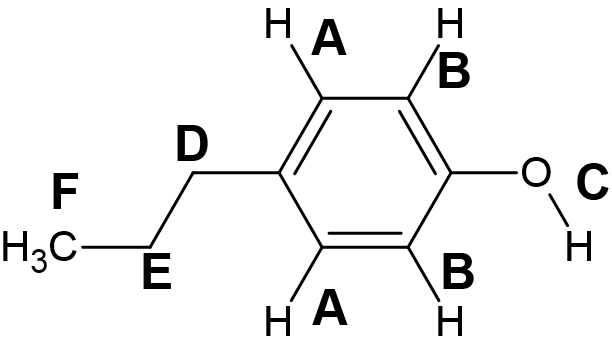
\includegraphics[width=0.33\textwidth]{img/struktur_linear_b.png}
	\caption{ermittelte Strukturformel (p-Propyphenol)}
	\label{fig:struktur_linear}
\end{figure}
\FloatBarrier

\subsection{Begründung der Probenstruktur}
Um weiter die Struktur in Abb. \ref{fig:struktur_linear} der unbekannten Probe begründen zu können, werden weitere Quellen hinzugezogen. In diesem Fall werden zwei recherchierte Spektren zum p-Propylphenol mit dem aufgenommenem Spektrum verglichen.
Zunächst wurde ein ${}^1$H-NMR-Spektrum mit Hilfe der Quelle \cite{Patiny.30.06.2021} simuliert. Auf der angegebenen Website lässt sich eine Struktur zeichnen oder Hochladen und infolgedessen ein Spektrum dazu simulieren. Zu beachten ist jedoch, dass auf der Website vermerkt ist, dass labile Protonen, wie in \ce{NH}-, \ce{CO2H}- oder \ce{OH-}Gruppen, nicht simuliert werden.
Das simulierte Spektrum ist in Abb. \ref{fig:spektrum_simuliert} zu sehen.
\begin{figure}[h!]
	\centering
	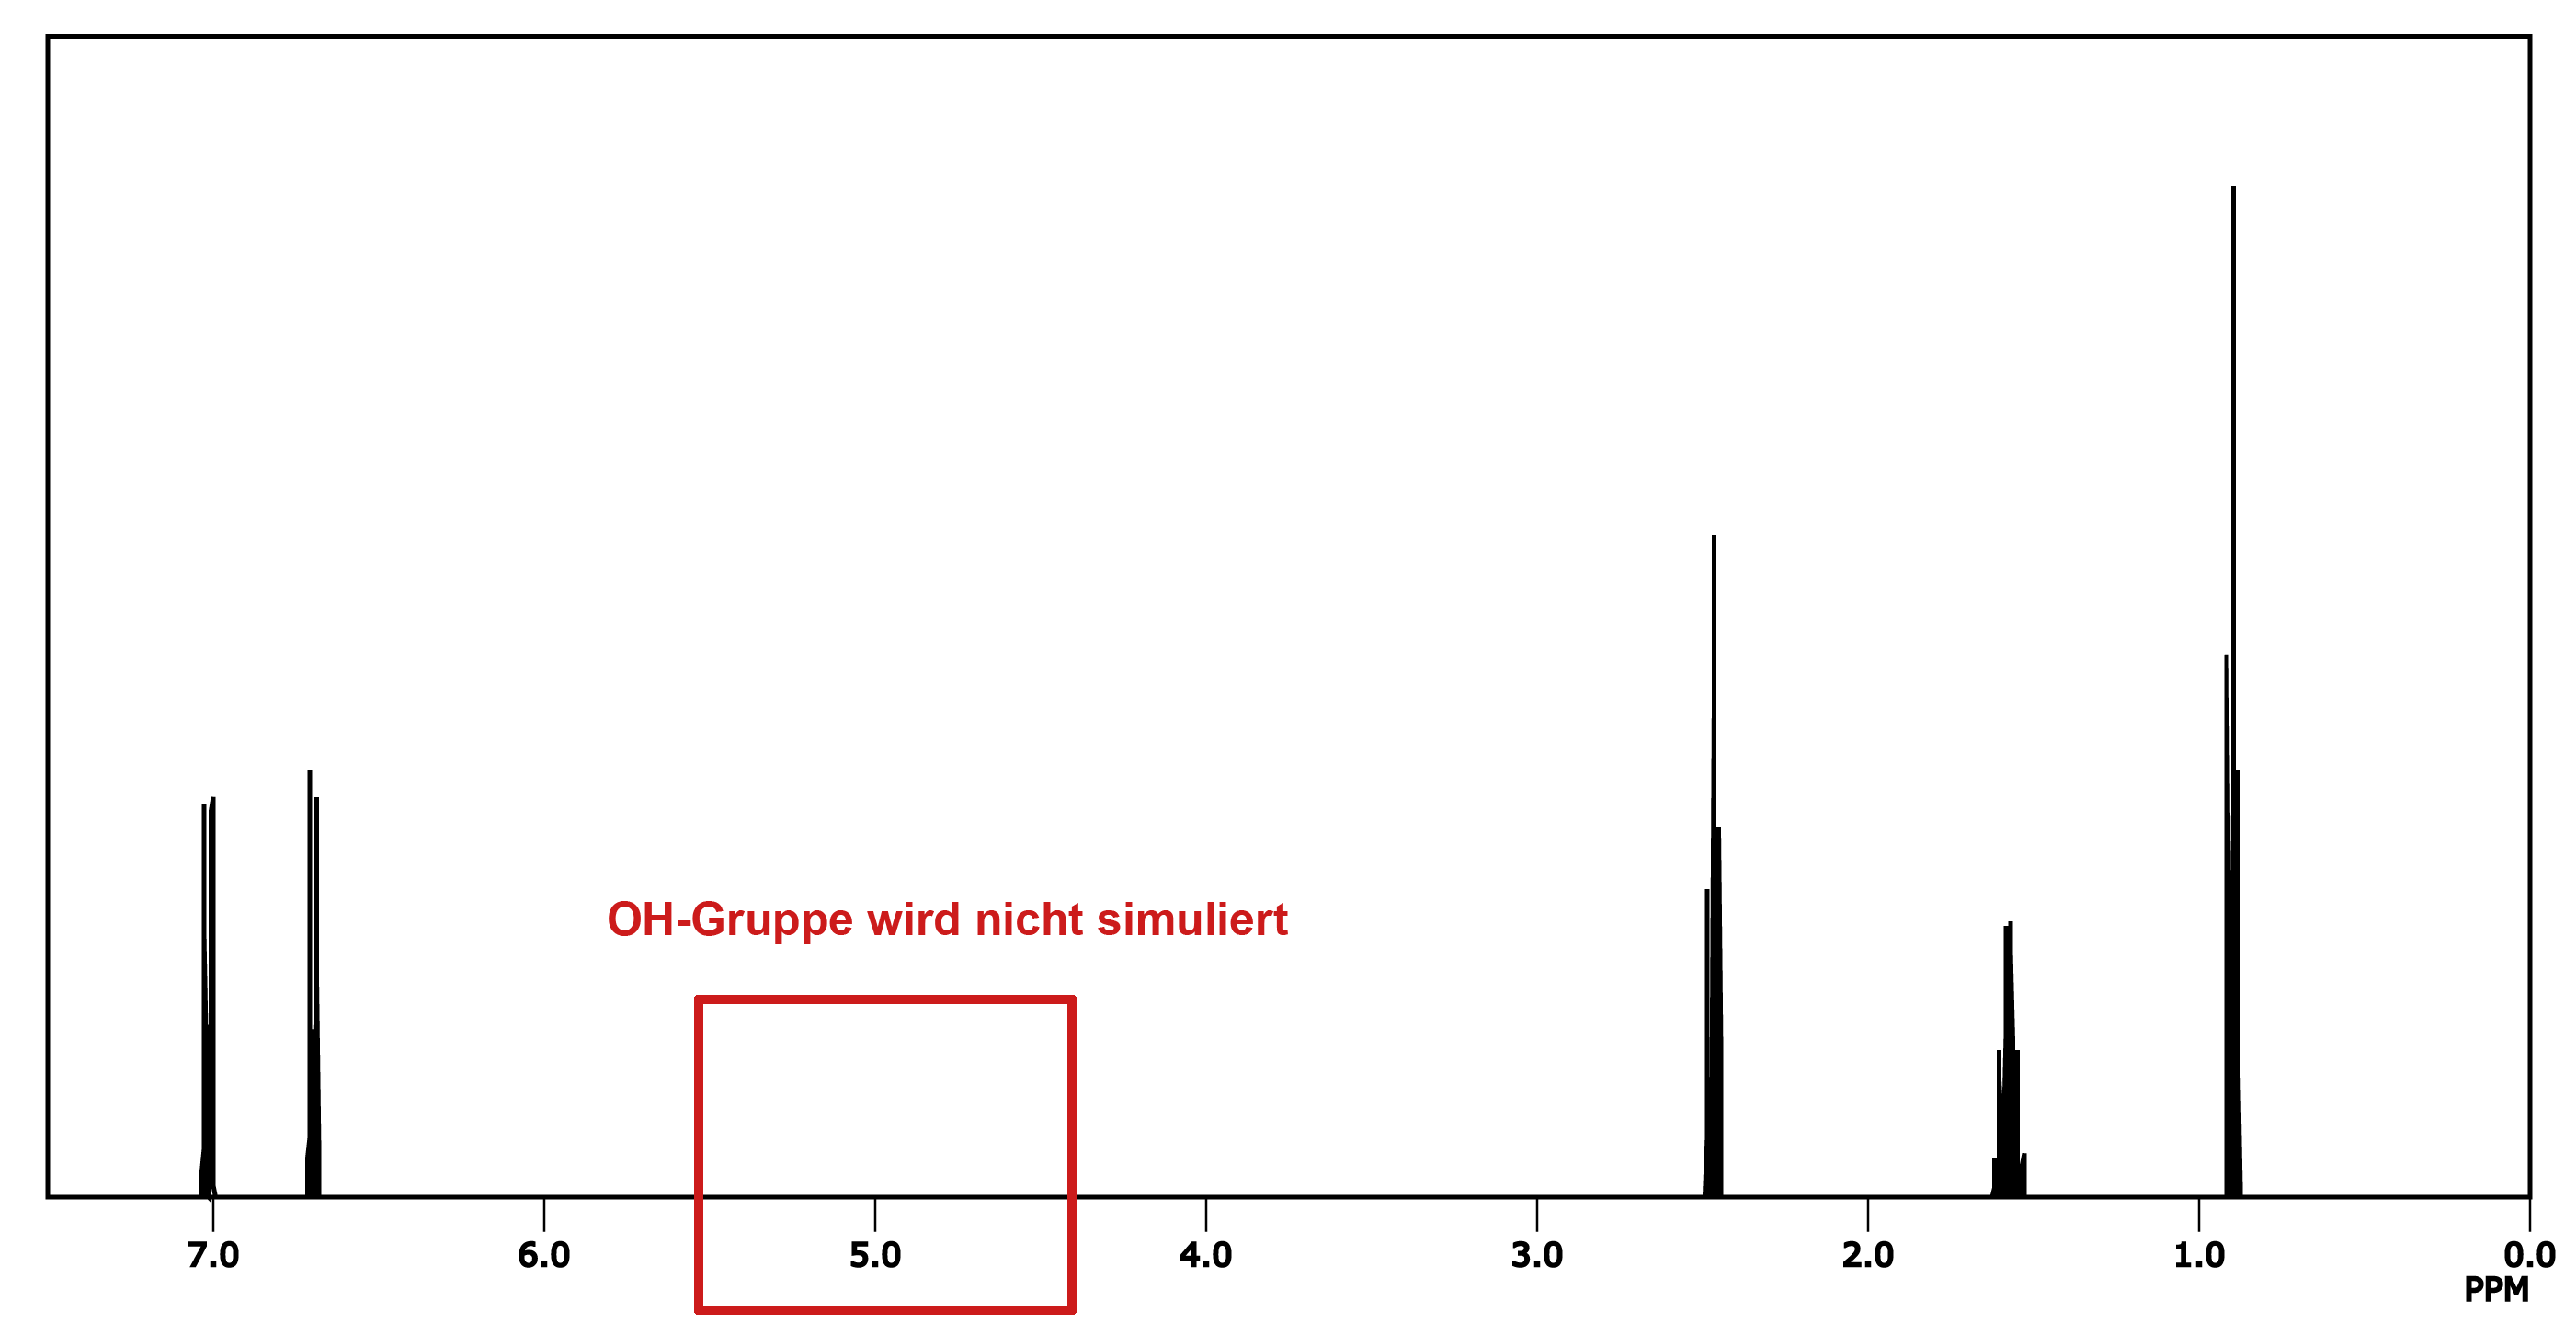
\includegraphics[width=\textwidth]{img/spektrum_simuliert_gesamt_oh.png}
	\caption{mit \url{www.nmrdb.org} simuliertes Spektrum von p-Propylphenol \cite{Patiny.30.06.2021}}
	\label{fig:spektrum_simuliert}
\end{figure}

Vergleicht man das simulierte Spektrum in Abb. \ref{fig:spektrum_simuliert} mit dem aufgenommen Spektrum in Abb. \ref{fig:spektrum_original} fällt auf, dass diese Spektren sich sehr ähnlich sind in Bezug auf die vorliegenden Kopplungsmuster. Weiterhin sind lediglich geringe Abweichungen in den chemischen Verschiebungen der Signale festzustellen. In der Anzahl der Messsignale unterscheiden sich jedoch beide Spektren, das die \ce{OH}-Gruppe des p-Propylphenols, wie zuvor beschrieben, nicht mit simuliert wird.
Lässt man den fehlenden \ce{OH}-Peak außer Acht begründetet das simuliert Spektrum bereits die bestimmte Struktur der Probe. 
\newpage
Weiterhin wird die Annahme, dass Peak F im originalen Spektrum ein Triplett ist, durch das simulierte Spektrum augenscheinlich bestätigt.\\
Um nicht nur ein simuliertes Spektrum als Rechtfertigung für die bestimmte Struktur in Abb. \ref{fig:struktur_linear} vorweisen zu können, wird zusätzlich eine Spektrendatenbank genutzt. In dieser wird konkret nach der bestimmten Struktur und dessen ${}^1$H-NMR-Spektrum gesucht. Vorteil einer solchen Datenbank ist es, dass die Verbindungen nicht simuliert, sondern real vermessen wurden. Die zu erwartenden Spektren sind demnach mit dem im Praktikum aufgenommen Spektrum besser zu vergleichen. Als NMR-Datenbank wurde die \textit{Spectral Database for Organic Compounds} alias \textit{SDBS} genutzt \cite{AIST.30.06.2021}. Das dort gefundene Spektrum für p-Propylphenol ist in Abbildung \ref{fig:spektrum_sdbs} dargestellt.

\begin{figure}[h!]
	\centering
	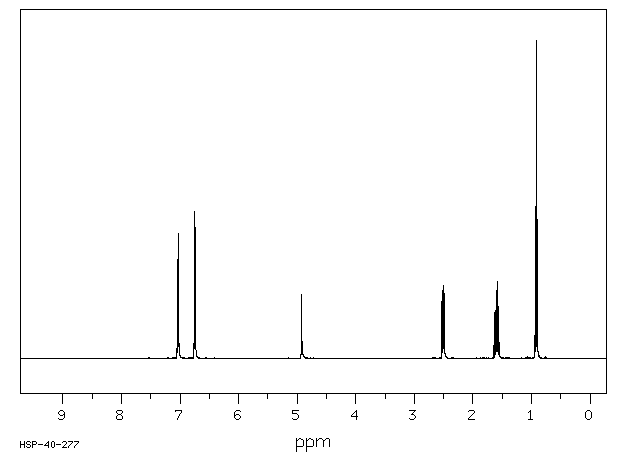
\includegraphics[width=0.75\textwidth]{img/sdbs_spektrum.png}
	\caption{Spektrum von p-Propylphenol aus der \textsc{AIST} SDBS-Datenbank \cite{AIST.30.06.2021}}
	\label{fig:spektrum_sdbs}
\end{figure}
\FloatBarrier

Auch in diesem Spektrum erscheinen die chemische Verschiebung, sowie das Kopplungsmuster sehr ähnlich zum selbst gemessenen Spektrum. Zudem fällt auf, dass im Vergleich zum simulierten Spektrum in Abb. \ref{fig:spektrum_simuliert} auch ein Peak für die  \ce{OH}-Gruppe zu verzeichnen ist. Mögliche Unterschiede könnten sich durch Signalrauschen oder leicht unterschiedliche Messbedingungen erklären lassen. Weiterhin ist auch in diesem Spektrum das äußerste Signal mit der kleinsten chemischen Verschiebung als Triplett zu charakterisieren.
Somit untermauert das Vergleichsspektrum für p-Propylphenol ebenfalls die bestimmte Struktur in Abb. \ref{fig:struktur_linear} des aufgenommenen Spektrums in \mbox{Abb. \ref{fig:spektrum_original}}. \\

Für die unbekannte Probe wird daher behauptet, dass es sich um die organische Verbindung p-Propylphenol alias 4-Propylphenol handelt.